\documentclass[aspectratio=169,10pt]{beamer}
\usetheme{default}
\usefonttheme{professionalfonts}
\usepackage{helvet}
\usepackage{booktabs}
\usepackage{tikz}
\usetikzlibrary{arrows.meta,positioning}
\renewcommand{\familydefault}{\sfdefault}
\definecolor{accent}{HTML}{087F8C}
\definecolor{accentdark}{HTML}{075B63}
\definecolor{ink}{HTML}{15242B}
\definecolor{muted}{HTML}{5F6F75}
\setbeamercolor{normal text}{fg=ink,bg=white}
\setbeamercolor{frametitle}{fg=ink,bg=white}
\setbeamercolor{structure}{fg=accent}
\setbeamertemplate{navigation symbols}{}
\setbeamertemplate{frametitle}{\vspace{0.3em}\insertframetitle\par\vspace{-0.2em}\color{accent}\rule{\textwidth}{0.6pt}}
\setbeamertemplate{footline}{\hfill\color{muted}\scriptsize CORE + LLM \quad \insertframenumber/\inserttotalframenumber\hspace{1.2em}\vspace{0.7em}}
\newcommand{\status}[1]{\textcolor{accentdark}{\textbf{#1}}}
\title{Pure-ID Session-based Recommendation with LLMs\\[0.35em]\Large Research Progress}
\subtitle{CORE + LLM Exploration}
\author{Way}
\date{October 5, 2026 -- Research meeting}
\begin{document}
\begin{frame}[plain]\titlepage\end{frame}

\begin{frame}{Research question}
\centering\Large\textbf{Can pretrained LLM sequence modeling transfer to pure-ID session recommendation?}
\vspace{1em}
\begin{enumerate}\normalsize
\item Can an LLM process learned item-ID embeddings?
\item Can it improve next-item ranking over CORE?
\item Does language pretraining itself add value?
\item Does value concentrate on unseen-in-session exploration?
\end{enumerate}
\vfill\status{Pure-ID: no names, brands, descriptions, or semantic metadata.}
\end{frame}

\begin{frame}{CORE + LLM architecture}
\centering
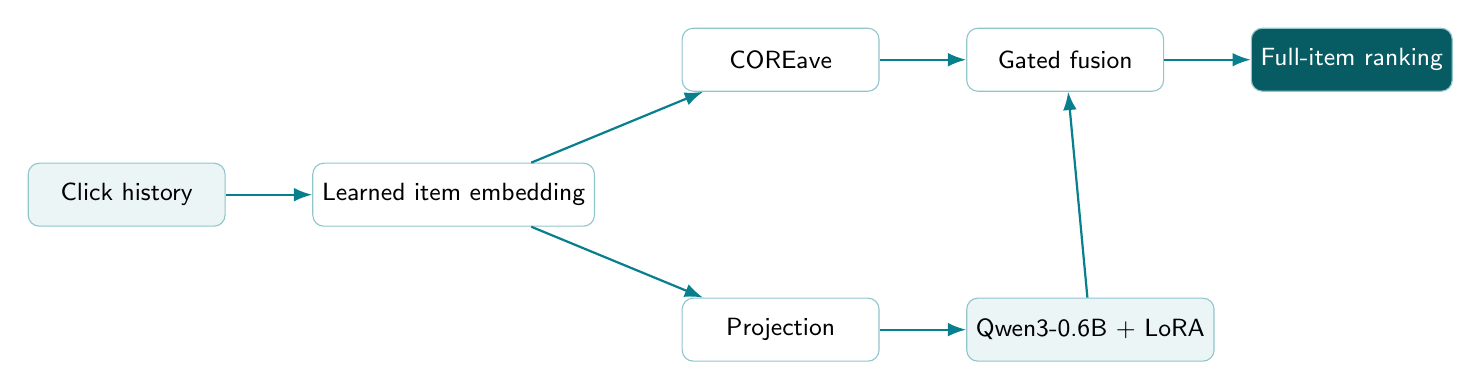
\begin{tikzpicture}[node distance=9mm and 11mm, every node/.style={font=\small}, box/.style={draw=accent!45,rounded corners,minimum height=8mm,minimum width=25mm,align=center}, arr/.style={-Latex,thick,draw=accent}]
\node[box,fill=accent!8] (hist) {Click history};
\node[box,right=of hist] (emb) {Learned item embedding};
\node[box,above right=of emb] (core) {COREave};
\node[box,below right=of emb] (proj) {Projection};
\node[box,fill=accent!8,right=of proj] (qwen) {Qwen3-0.6B + LoRA};
\node[box,right=of core] (gate) {Gated fusion};
\node[box,fill=accentdark,text=white,right=of gate] (rank) {Full-item ranking};
\draw[arr] (hist)--(emb); \draw[arr] (emb)--(core); \draw[arr] (emb)--(proj); \draw[arr] (proj)--(qwen); \draw[arr] (core)--(gate); \draw[arr] (qwen)--(gate); \draw[arr] (gate)--(rank);
\end{tikzpicture}
\vfill\textbf{Continuous learned embeddings enter through \texttt{inputs\_embeds}. Item IDs never become text tokens.}
\end{frame}

\begin{frame}{Experimental setup}
\begin{tabular}{ll}\toprule Setting & Value\\\midrule
Dataset & Tmall\\
Train / valid / test & 275,356 / 50,579 / 101,862\\
Items & 37,367 including padding\\
Max session length & 50\\
Metrics & Recall@10/20, MRR@10/20\\
Selection & Valid MRR@20\\\bottomrule
\end{tabular}
\vspace{1em}
\textbf{Models:} COREave, COREtrm, CORE + Qwen3-0.6B + LoRA\\
\status{Single-seed preliminary validation comparison. No matched full test result yet.}
\end{frame}

\begin{frame}{Current result}
\centering
\begin{tabular}{lrr}\toprule Model & Recall@20 & MRR@20\\\midrule
COREave & 0.3471 & 0.1936\\
COREtrm & 0.3457 & 0.1936\\
CORE + LLM & 0.3414 & 0.1896\\\bottomrule
\end{tabular}
\vspace{1.1em}
{\Huge\textcolor{accentdark}{\textbf{-2.07\%}}}\\
LLM vs CORE on MRR@20\\[0.8em]
\textbf{Current default configuration does not outperform CORE.}\\[0.8em]
\small Diagnostic: Recall@20 reached 0.3570 at epoch 3, while MRR@20 fell to 0.1868.
\end{frame}

\begin{frame}{Current findings}
\begin{columns}[T]
\column{0.31\textwidth}\textcolor{accentdark}{\Large\textbf{Engineering}}\\Pure-ID embeddings pass through Qwen. The full training and validation pipeline works.
\column{0.31\textwidth}\textcolor{accentdark}{\Large\textbf{Quality}}\\The current model trails matched CORE baselines on validation MRR@20.
\column{0.31\textwidth}\textcolor{accentdark}{\Large\textbf{Attribution}}\\Pretraining and architecture remain confounded. The full random-backbone control is untested.
\end{columns}
\vfill\status{This experiment tests direct representation transfer. Explicit intent reasoning remains untested.}
\end{frame}

\begin{frame}{Representation mismatch}
\centering\Large\textbf{A pretrained language model receives a completely new alphabet}
\vspace{1em}
\begin{columns}
\column{0.34\textwidth}\centering\textbf{Language pretraining}\\words\\syntax\\semantic structure
\column{0.28\textwidth}\centering\status{representation mismatch}
\column{0.34\textwidth}\centering\textbf{Pure-ID input}\\arbitrary labels\\learned vectors\\behavioral signal only
\end{columns}
\vfill\textbf{Preliminary implication:} sequence ability may require behavioral structure or task specialization before it transfers.
\end{frame}

\begin{frame}{Compute consideration}
\begin{tabular}{lr}\toprule Model & Recorded seconds / epoch\\\midrule
COREave & 47.20\\
COREtrm & 100.91\\
Qwen + LoRA & 3538.43\\\bottomrule\end{tabular}
\vspace{1em}
{\Huge\textcolor{accentdark}{\textbf{75$\times$}}} slower than COREave in recorded training time.\\[1em]
\status{Recorded training cost must be considered alongside ranking quality.}
\end{frame}

\begin{frame}{Immediate plan}
\textbf{Now:} diagnose gate and branch behavior, run matched learning-rate searches, add a random-backbone control, and validate paired seeds.\\[1.2em]
\textbf{If a stable positive signal appears:} paired seeds, random-backbone control, locked final-test evaluation.\\[1.2em]
\textbf{If no stable gain appears:} shrink the LLM direction.\\[1.5em]
\status{Next-stage goal: identify where LLM reasoning adds measurable value before increasing model size.}
\end{frame}
\end{document}
